\begin{figure}[ht!]
  \centering
  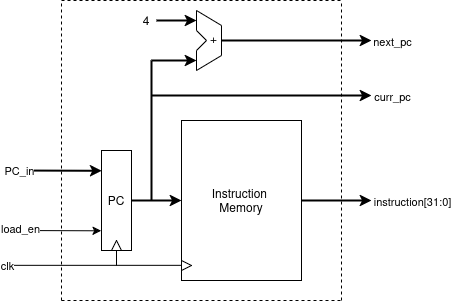
\includegraphics[scale = 0.4]{IF_BD.png}
  \caption{Basic instruction fetch block diagram}
  \label{fig:IF_BD}
\end{figure}
\subsection{Basic description}
This stage of the datapath fetches the instruction to be executed, which is stored in the Instruction Memory. This memory can be implemented using Vivado's Block Memory Generator IP, configured as a single-port RAM with a 32-bit read-write width. The memory size should be addressable using at least 12 bits, because the AUIPC instruction must be able to load absolute addresses that are shifted by that amount into the Program Counter (PC).
The Program Counter is a register that holds the address of the current instruction and, during program execution, the latter is incremented at each rising edge of the clock; Since memory is byte-addressable and each instruction is 4 bytes long, the PC is incremented by 4 at each step. 
In this project, however, the Instruction Memory is simulated using a RAM with 32-bit words per address; While the architecture should still work with bytes, the increment is going to remain 4, but the two least significant bits of the address shall be unused from now on.
To handle jumps or branches in the program, the PC may accept another value as input from a different stage along the datapath, allowing it to be loaded with a new address after such instructions are executed.
In VHDL, a register can be synthesized by declaring a clock-dependent (and in this case also \emph{load{\_}en} dependent) \emph{signal}, hence the PC will be implemented with this method.
A VHDL entity that describes this stage can be defined as follows:\\
\begin{minted}[fontsize=\footnotesize]{vhdl}
entity instr_fetch is
 port ( 
  clk        : in std_logic;
  pc_load_en : in std_logic;
  pc_in      : in std_logic_vector(11 downto 0);

  next_pc    : out std_logic_vector(11 downto 0);
  curr_pc    : out std_logic_vector(11 downto 0);
  instr      : out std_logic_vector(31 downto 0)
  );
end instr_fetch;
\end{minted}
\vspace{1\baselineskip}
With the previously specified settings, the IP used for the Instruction Memory will generate a component that can be instantiated in the architecture as follows:\\
\begin{minted}[fontsize=\footnotesize]{vhdl}
component instruction_memory
 port(
  clka  : in std_logic;
  wea   : in std_logic;
  addra : in std_logic_vector(9 downto 0);
  dina  : in std_logic_vector(31 downto 0);
  douta : out std_logic_vector(31 downto 0));
end component;
\end{minted}
\vspace{1\baselineskip}

The inputs \emph{wea} (i.e. the write-enabling input) and \emph{dina} (data input) will be pulled low since there is no need for the moment to write inside the memory. 
Since the PC has to act as a pointer for the instruction, its output will be routed to the \emph{addra} input, excluding the first two least significant bits in order to proceed 32 bits (the length of a standard instruction) at a time.
With this being said, the only thing that is left to do is a clock-sensitive process that increments the PC or loads another address from the outside if the load-enable input of its register is pulled high. 
By implementing the register as a \emph{signal} named \emph{pc{\_}reg}, the resulting VHDL script for the architecture is shown in Source Code \ref{code:IF_code}.


\subsection{Simulation}
A testbench for this simulation will require the PC to be incremented by 4 so that every location in the memory is addressed, but in order to actually see a stream of instructions at the output a .coe file for the initialization of the instruction memory is required:

\begin{minted}{text}
  memory_initialization_radix=16;
  memory_initialization_vector=
  00000293,     --> addi x5, x0, 0
  00100313,     --> addi x6, x0, 1
  005303B3;     --> add x7, x6, x5
\end{minted}
A .coe file requires the hexadecimal dump of the program, in this given example each instruction has its assembly equivalent on the right.\\
For the testbench, a simple clock can be simulated with a process while a small register can be simulated for storing \emph{next{\_}pc} and re-routing its value on \emph{pc{\_}in}, hence the testbench, shown in Code \ref{code:IF_TB} gives the resulting behavior:

\begin{figure}[h!]
  \centering
  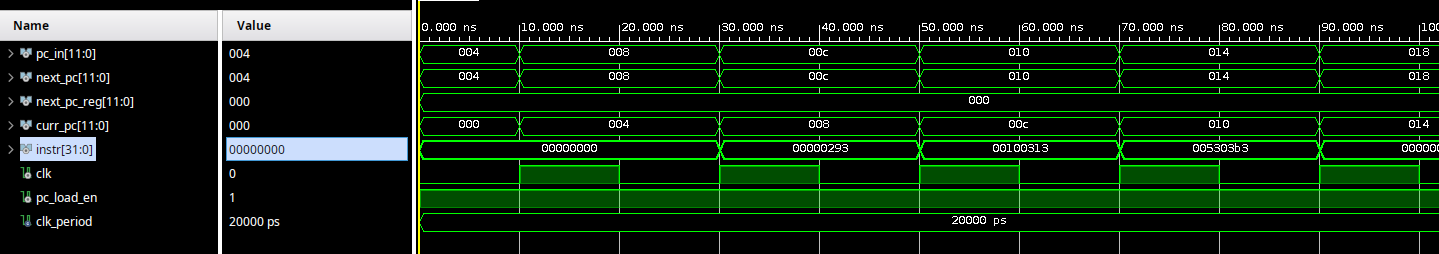
\includegraphics[scale = 0.45]{IF_sim.png}
\end{figure}

The results state that \emph{curr{\_}pc}, in fact, acts as a register, refreshed as the clock's rising edge approaches, and the flow of instructions are the same as the ones stated in the \emph{.coe} file. 
